\section{Technischer Entwurf}
\subsection{Grundlegende Architektur}
In Abbildung \vref{fig:Aufbau} ist der grundlengede Aufbau der Webanwendung skizziert.
Dieser besteht aus mehreren Komponenten, die gemäß eines Microservice-Ansatzes unabhängig voneinander bestehen. 
Dies bietet außerdem die Vorteile, dass durch die verringerte Kopplung eine bessere Wartbarkeit der einzelnen Bestandteile gegeben ist sowie diese einfach ersetzt werden können. 
Mithilfe eines Docker-Netzwerks kann dieser Ansatz umgesetzt werden und bietet zusätzlich ein einfaches Deployment der Anwendung. 

\begin{figure}[H]
	\centering 
	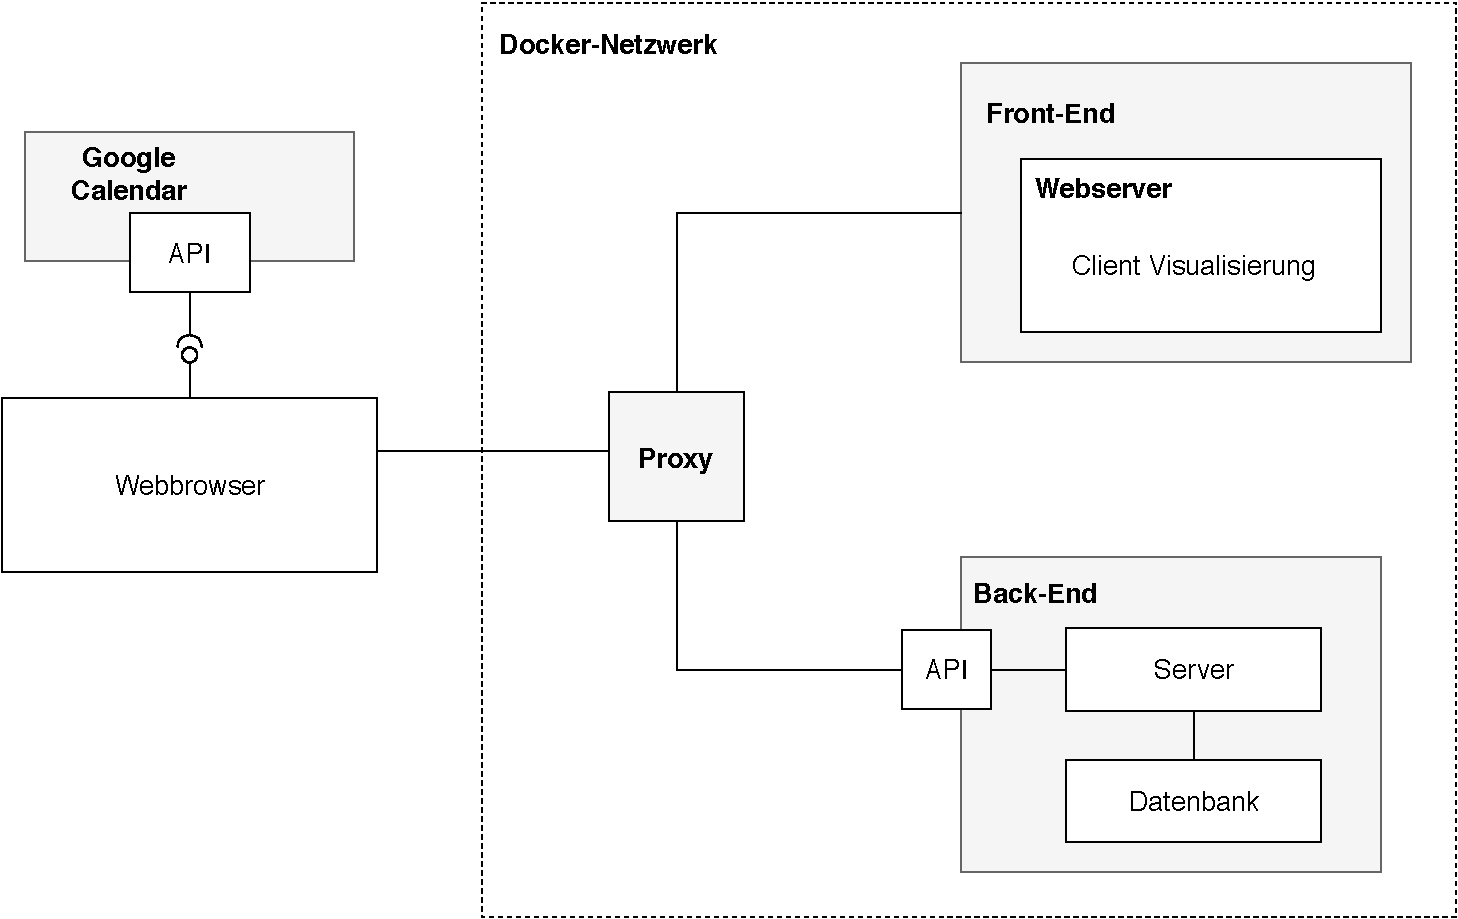
\includegraphics[width=13cm]{img/TechnischerEntwurf.pdf}
	\caption[Grundlegende Architektur]{\label{fig:Aufbau}Grundlegende Architektur}
\end{figure}

Die Abbildung stellt eine Übersicht über den Aufbau dar und bietet eine logische Trennung der Komponenten. 
Allgemein lassen sich folgende Hauptkomponenten unterscheiden:
\begin{itemize}
    \item Front-End zur Bereitstellung der Benutzeroberfläche an den Webbrowser des Clients 
    \item Back-End zur Datenhaltung und Geschäftslogik
    \item Proxy als Kommunikationsschnittstelle
    \item Webbrowser mit einer Anbindung an die Google Calendar-Schnittstelle.
\end{itemize} 

Das Front- und Back-End sollen als eigenständige Microservices mit eigenem Server umgesetzt werden, sodass die Entwicklung der Komponenten losgelöst ablaufen kann und durch andere Technologien ersetzt werden könnte.
Das Front-End dient zur Bereitstellung der grafischen Benutzeroberfläche und wird an den Webbrowser des Clients ausgeliefert. 
Das Back-End hingegen besteht aus einem Server mit der Geschäftslogik sowie einer Datenbank zur Datenhaltung der Anwendung. 
Diese Dienste sollen über eine \ac{API} erreichbar sein. 
Der Proxy stellt die zentrale Schnittstelle der Webanwendung dar und liefert das Front-End aus. 
Von dem Webbrowser wird außerdem auf die externe Schnittstelle des Google Calendars zugegriffen, um eine Verbindung zu einem Google Calendar gemäß der Anforderung A2 und A3 aus der Tabelle \vref{anf:GC} herzustellen.


\subsection{Datenmodell}
Für das serverseitige Speichern von Daten sind relationale Datenbanken weit verbreitet.
Deshalb wird auch im Rahmen dieses Projekts eine solche Form der Datenhaltung genutzt.
Im Folgenden wird nun das Datenmodell näher erläutert, welches im Anhang \ref{fig:ermodell} dargestellt ist.  

Über \texttt{directorOfStudies} werden die Nutzer der Anwendung, die Studiengangsleiter, dargestellt.
Sie sind nicht automatisch als Dozenten hinterlegt, können jedoch als solche hinzugefügt werden.
Ein Studiengangsleiter kann zusätzlich ein Administrator der Anwendung sein, wodurch er weitere Berechtigungen erhält, wie das Zurücksetzen von Passwörtern.

Die Entität \texttt{course} repräsentiert einen Kurs der \ac{DHBW}, welcher genau einem Studiengang (\texttt{fieldOfStudy}) und einer Studienrichtung (\texttt{majorSubject}) zugeordnet ist.
Damit die Eindeutigkeit der Module (Anforderung \hyperref[tab:Anforderungen]{A7}) gewährleistet ist, referenziert \texttt{majorSubject} auf die dazugehörigen Modulgruppen und entspricht dadurch dem gegebenen Aufbau des Modulkatalogs.
Aus diesem Grund beinhaltet es auch das Jahr, ab welchem der Modulkatalog gültig ist. 

Damit auch Wahlmodule abgebildet werden können (Anforderung \hyperref[tab:Anforderungen]{A24}), sind die Module (\texttt{module}) Teil einer Modulgruppe (\texttt{moduleGroup}).
Besteht die Wahlmöglichkeit zwischen mehreren Modulen, beinhaltet die Modulgruppe alle wählbaren Module.
Andernfalls beinhaltet sie nur das vorgesehene Modul.
Damit neben den Informationen des aktuellen Modulkatalogs der \ac{DHBW} auch die Prüfungsleistung je Modul gespeichert werden kann, wird die Entität \texttt{academicRecord} verwendet.

Kurse beinhalten neben ihrem Namen auch eine Referenz auf den für sie angelegten Google Calendar. 
Mithilfe von \texttt{semester} werden die kursspezifischen Semester festgelegt, welche den zeitlichen Rahmen des Studiums beschreiben.
Die Kurse unterliegen üblicherweise einem Studiengangsleiter, jedoch ist es auch möglich weitere Studiengangsleiter hinzuzufügen, bspw. für Übergangszeiten bei Positionswechseln.

Die Dozenten (\texttt{lecturer}) werden durch zahlreiche Attribute beschrieben (Anforderung \hyperref[tab:Anforderungen]{A10}) sowie ein Lebenslauf kann als PDF gesondert gespeichert werden.
Gemäß Anforderung \hyperref[tab:Anforderungen]{A1} findet die Verwaltung der Dozenten in einem zentralen Dozentenpool statt.
Dabei ist ihnen jeweils genau ein Studiengangsleiter als Ersteller zugeordnet (Anforderung \hyperref[tab:Anforderungen]{A12}) und die Bearbeitbarkeit durch andere Studiengangsleiter kann eingeschränkt werden. 
Für die Verknüpfung zwischen Dozierenden und Vorlesung wird ein thematischer Schwerpunkt (\texttt{mainFocus}) eingesetzt.
Dadurch wird es ermöglicht passende Dozenten für Vorlesungen vorzuschlagen (Anforderung \hyperref[tab:Anforderungen]{A25}).

Eine \texttt{lecture} ist eine abstrakte Lehr-/Lerneinheit.
Sie beinhaltet lediglich allgemeine Beschreibungen und ist somit für alle Kurse einer Studienrichtung anwendbar. 
Planungseinheiten für konkrete Veranstaltungen werden über die Entität \texttt{presentations} abgebildet.
Sie referenzieren auf abstrakte Vorlesungen, eine Prüfungsleistung sowie ein Semester und einen Kurs. 
Durch Planungseinheiten können gleiche Veranstaltungen mehrfach erzeugt werden, um mehrere Dozenten gleichzeitig zu kontaktieren und anzufragen.
Der Status einer \texttt{presentation} indiziert den Fortschritt der Planung und die Rückmeldungen der jeweiligen Dozenten.
